\chapter{Izvedba}

Sustav kreiran kao prakti\v{c}ni dio ovoga rada se sastoji od mobilne i internetske aplikacije te je shodno tome ovo poglavlje podjeljeno na dva dijela u kojima su opisane korit\v{s}tene tehnologije i alati, te motivi za odabir istih. Iako su aplikacije iz razli\v{c}itih podru\v{c}ja ra\v{c}unarstva, razvoj im je organiziran i vo\dj en na isti nain, koriste\'{c}i alat Git \cite{git}. Git je alat kojeg je kreirao tim Linusa Torvaldsa (otac Linuxa i jedan od najbitnijih i zna\v{c}ajniji u ra\v{c}unarstvu uop\'{c}e) za potrebe razvoja jezgre Linux-a. Git slu\v{z}i za verzioniranje i organizaciju koda i funkcionira na na\v{c}in da korisnik grupira napravljene promjene u cjeline (commit-ove) koji \v{c}ine logi\v{c}ke cjeline (branch-eve) koje obi\v{c}no predstavljaju funkcionalnosti aplikacije. Na taj na\v{c}in je cijeli razvoj projekta evidentiran i u bilo kojem trenutku se mo\v{z}e vratiti na neko pro\v{s}lo stanje. Posebno je koristan u organizaciji timova od vi\v{s}e ljudi jer omogu\'{c}ava da vi\v{s}e ljudi radi na razl\v{c}iitim djelovima projketa (\v{c}ak i na istom kodu jer posjeduje mehanizam za rje\v{s}avanje konflikata nastalih ure\dj enjem iste linije koda od vi\v{s}e programera). U praksi se koriste i razli?ite metode kori\v{s}tenja Git-a, od kojih je naj\'{c}e\v{s}\'{c}e kori\v{s}tena ``Git flow?? \cite{git_flow}, koja specificira organizaciju branch-eva s ciljem standardizacije i efektivnijeg kori\v{s}tenja Git-a. Nadalje, u praksi se Git koristi u kombinaciji sa platformama za pohranjivanje projekata \v{s}to omogu\'{c}uje decentralizaciju projekta, kolaboraciju vi\v{s}e programera i sigurnost (rezervna kopija je serveru). Oba projekta koriste platformu Github \cite{github} koja je jedna od najkori\v{s}tenijih platformi za projekte otvorenog koda. Uz navedene prednosti, Github pru\v{z}a i dodatne statistike i informacije o projektu, kao npr. aktivnost graf napravljenih commitova u vremenu, prikazan na slici  ~\ref{fig:commits}.

\begin{figure}[!htbp]
	\begin{center}
 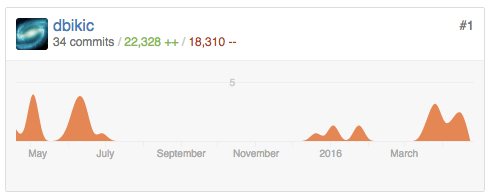
\includegraphics[height=4.2cm,keepaspectratio=true]{git_commits}
 \caption{Graf commit-ova u vremenskom periodu za projekt mobilne aplikacije}
 \label{fig:commits}
	\end{center}
\end{figure}

\section{Internetska aplikacija}

\subsection{Tehnologije}

Internetska aplikacija se sastoji od dva dijela: klijentskog i poslu\v{z}iteljskog. Iako se oba dijela nalaze na istom poslu\v{z}itelju, razlika izme\dj u njih je u lokaciji na kojoj se kod izvr\v{s}ava. Klijentski dio se izvr\v{s}ava u korisni\v{c}kom pregledniku te on uklju\v{c}uje korisni\v{c}ko su\v{c}elje aplikacije, dok se poslu\v{z}iteljski dio izvr\v{s}ava na poslu\v{z}itelju te on uklju\v{c}uje bazu podataka, su\v{c}elje za pristupanje istoj.

Korisni\v{c}ko su\v{c}elje je kreirano uz pomo\'{c} tri standardne internetske tehnologije koje su temelj interneta kakav je danas: HTML, CSS i Javascript. HTML \cite{html} (Hyper Text Markup Language) je standardni jezik za kreaciju elemenata internetske stranice i temelj za sav daljnji dizajn i logiku. CSS \cite{css} (Cascading Style Sheets) slu\v{z}i za definiranje stilova koji se dodaju HTML elementima i koje preglednik interpretira te na temelju njih definira izgled, poziciju i pona\v{s}anje elemenata. Javascript \cite{javascript} se koristi za interakciju korisnika i internetske stranice, te za manipulaciju HTML elemenata.

Poslu\v{z}iteljska strana uklju\v{c}uje MySQL bazu podataka i PHP skripte koje dohva\'{c}aju podatke iz iste te ih u obliku HTML elemenata prikazuju na korisni\v{c}kom su\v{c}elju. MySQL je sustav za upravljanje bazama podataka koji uklju\v{c}uje relacijsku bazu podataka kojojm se upravlja pomo\'{c}u SQL (Structured Querry Language) jezika. PHP (Hypertetxt Preprocessor) je skriptni jezik koji se koristi na poslu\v{z}iteljskoj strani za komunikaciju sa bazom. Funkcionira tako da se u HTML kod ugra\dj uje skriptni kod kojeg poslu\v{z}itelj prepoznaje i izvr\v{s}ava, te se rezultat izvr\v{s}avanja ispisuje u HTML kod koji se onda \v{s}alje klijentu.

Opisane tehnologije su izabrane prvenstveno zato jer su sve otvorenog koda, a zatim jer su standard u domeni internetskih aplikacija (HTML, CSS, Javascript) i jer im je primjena ra\v{s}irena i \v{c}esto se koriste u praksi (MySQL, PHP).

\subsection{Alati}
Kori\v{s}teni alati za izradu internetske aplikacije su:
\begin{itemize}
	\item Atom 1.6.2 \cite{atom}
	\begin{itemize}
		\item Ure\dj iva\v{c} koda razvijen od tvrtke GitHub
		\item Kori\v{s}ten za pisanje svog koda (HTML, CSS, Javascript i PHP)
	\end{itemize}
	
	\item XAMPP 5.6.12-0 \cite{xampp}
	\begin{itemize}
		\item Paket alata namjenjen za poslu\v{z}itelje koji uklju\v{c}uje HTTP poslu\v{z}itelj, MySQL bazu podataka i interpreter programskih jezika PHP i Pearl
		\item Kori\v{s}ten je za kreiranje lokalnog testnog poslu\v{z}itelja i za kreiranje i administraciju baze podataka pomo\'{c}u alata phpMyAdmin
	\end{itemize}
	
	\item FileZilla 3.16.1 \cite{filezilla}
	\begin{itemize}
		\item Klijent za SFTP (Secure File Transfer Protocol) prijenos datoteka na poslu\v{z}itelj
	\end{itemize}
\end{itemize}


\section{Mobilna aplikacija}

\subsection{Tehnologija}


\subsection{Alati}
Android studio



